\def \nbclasses {11}
\def \nbviewgraphdata {45/0.67205/0/0/369/817,15/0.38277/1/0/126/860,8/0.28832/2/0/68/818,4/0.20325/3/0/34/823,3/0.16151/4/0/21/805,4/0.20975/5/0/37/841,25/0.49676/6/0/210/851,16/0.39606/7/0/128/816,13/0.35464/8/0/102/811,9/0.29307/9/0/70/815,38/0.61926/10/0/311/811,5/0.21848/0/1/39/817,11/0.33236/1/1/95/860,16/0.40323/2/1/133/818,4/0.19408/3/1/31/823,4/0.20851/4/1/35/805,3/0.17583/5/1/26/841,10/0.31604/6/1/85/851,14/0.37048/7/1/112/816,7/0.272/8/1/60/811,5/0.21307/9/1/37/815,15/0.38786/10/1/122/811,11/0.33739/0/2/93/817,35/0.58964/1/2/299/860,42/0.64755/2/2/343/818,13/0.35377/3/2/103/823,1/0.09325/4/2/7/805,2/0.13793/5/2/16/841,20/0.44563/6/2/169/851,28/0.52511/7/2/225/816,34/0.57913/8/2/272/811,12/0.35028/9/2/100/815,10/0.31991/10/2/83/811,10/0.31681/0/3/82/817,12/0.34439/1/3/102/860,13/0.36167/2/3/107/818,48/0.69454/3/3/397/823,0/0.049844/4/3/2/805,0/0/5/3/0/841,11/0.3252/6/3/90/851,12/0.34832/7/3/99/816,17/0.41696/8/3/141/811,35/0.58927/9/3/283/815,6/0.24073/10/3/47/811,0/0.060597/0/4/3/817,0/0/1/4/0/860,1/0.11057/2/4/10/818,0/0.049296/3/4/2/823,61/0.7786/4/4/488/805,42/0.6497/5/4/355/841,1/0.076651/6/4/5/851,0/0.049507/7/4/2/816,2/0.136/8/4/15/811,0/0.035028/9/4/1/815,0/0.04966/10/4/2/811,1/0.085697/0/5/6/817,1/0.083527/1/5/6/860,1/0.098894/2/5/8/818,0/0.034858/3/5/1/823,24/0.49091/4/5/194/805,46/0.67923/5/5/388/841,1/0.096957/6/5/8/851,2/0.14003/7/5/16/816,1/0.092905/8/5/7/811,1/0.078326/9/5/5/815,1/0.092905/10/5/7/811,4/0.19479/0/6/31/817,5/0.21567/1/6/40/860,4/0.18829/2/6/29/818,6/0.23897/3/6/47/823,0/0.035245/4/6/1/805,1/0.077106/5/6/5/841,5/0.22216/6/6/42/851,5/0.23221/7/6/44/816,2/0.13139/8/6/14/811,3/0.16052/9/6/21/815,6/0.24073/10/6/47/811,6/0.24985/0/7/51/817,6/0.24825/1/7/53/860,5/0.21268/2/7/37/818,5/0.21769/3/7/39/823,0/0/4/7/0/805,0/0.034483/5/7/1/841,6/0.24239/6/7/50/851,6/0.25485/7/7/53/816,8/0.28527/8/7/66/811,5/0.22154/9/7/40/815,4/0.19233/10/7/30/811,14/0.3719/0/8/113/817,10/0.3217/1/8/89/860,6/0.24723/2/8/50/818,2/0.14372/3/8/17/823,1/0.086333/4/8/6/805,0/0/5/8/0/841,16/0.39681/6/8/134/851,12/0.34478/7/8/97/816,12/0.34226/8/8/95/811,4/0.18863/9/8/29/815,12/0.35115/10/8/100/811,1/0.07823/0/9/5/817,2/0.1364/1/9/16/860,1/0.085644/2/9/6/818,11/0.33252/3/9/91/823,0/0/4/9/0/805,0/0/5/9/0/841,3/0.1714/6/9/25/851,1/0.099015/7/9/8/816,0/0.070229/8/9/4/811,20/0.44858/9/9/164/815,3/0.17905/10/9/26/811,3/0.17493/0/10/25/817,4/0.19883/1/10/34/860,3/0.18168/2/10/27/818,7/0.27225/3/10/61/823,6/0.2517/4/10/51/805,2/0.12433/5/10/13/841,4/0.19692/6/10/33/851,4/0.19803/7/10/32/816,4/0.20774/8/10/35/811,8/0.28241/9/10/65/815,4/0.21069/10/10/36/811}
\def \nbviewgraphlabels {Plywood1/0,Plywood2/1,Drywall1/2,Drywall2/3,Metal1/4,Metal2/5,Foam1/6,Foam2/7,Glass1/8,Glass2/9,LOS/10}
\def \titletext {Entire dataset with noise reduction [27 percent success]}
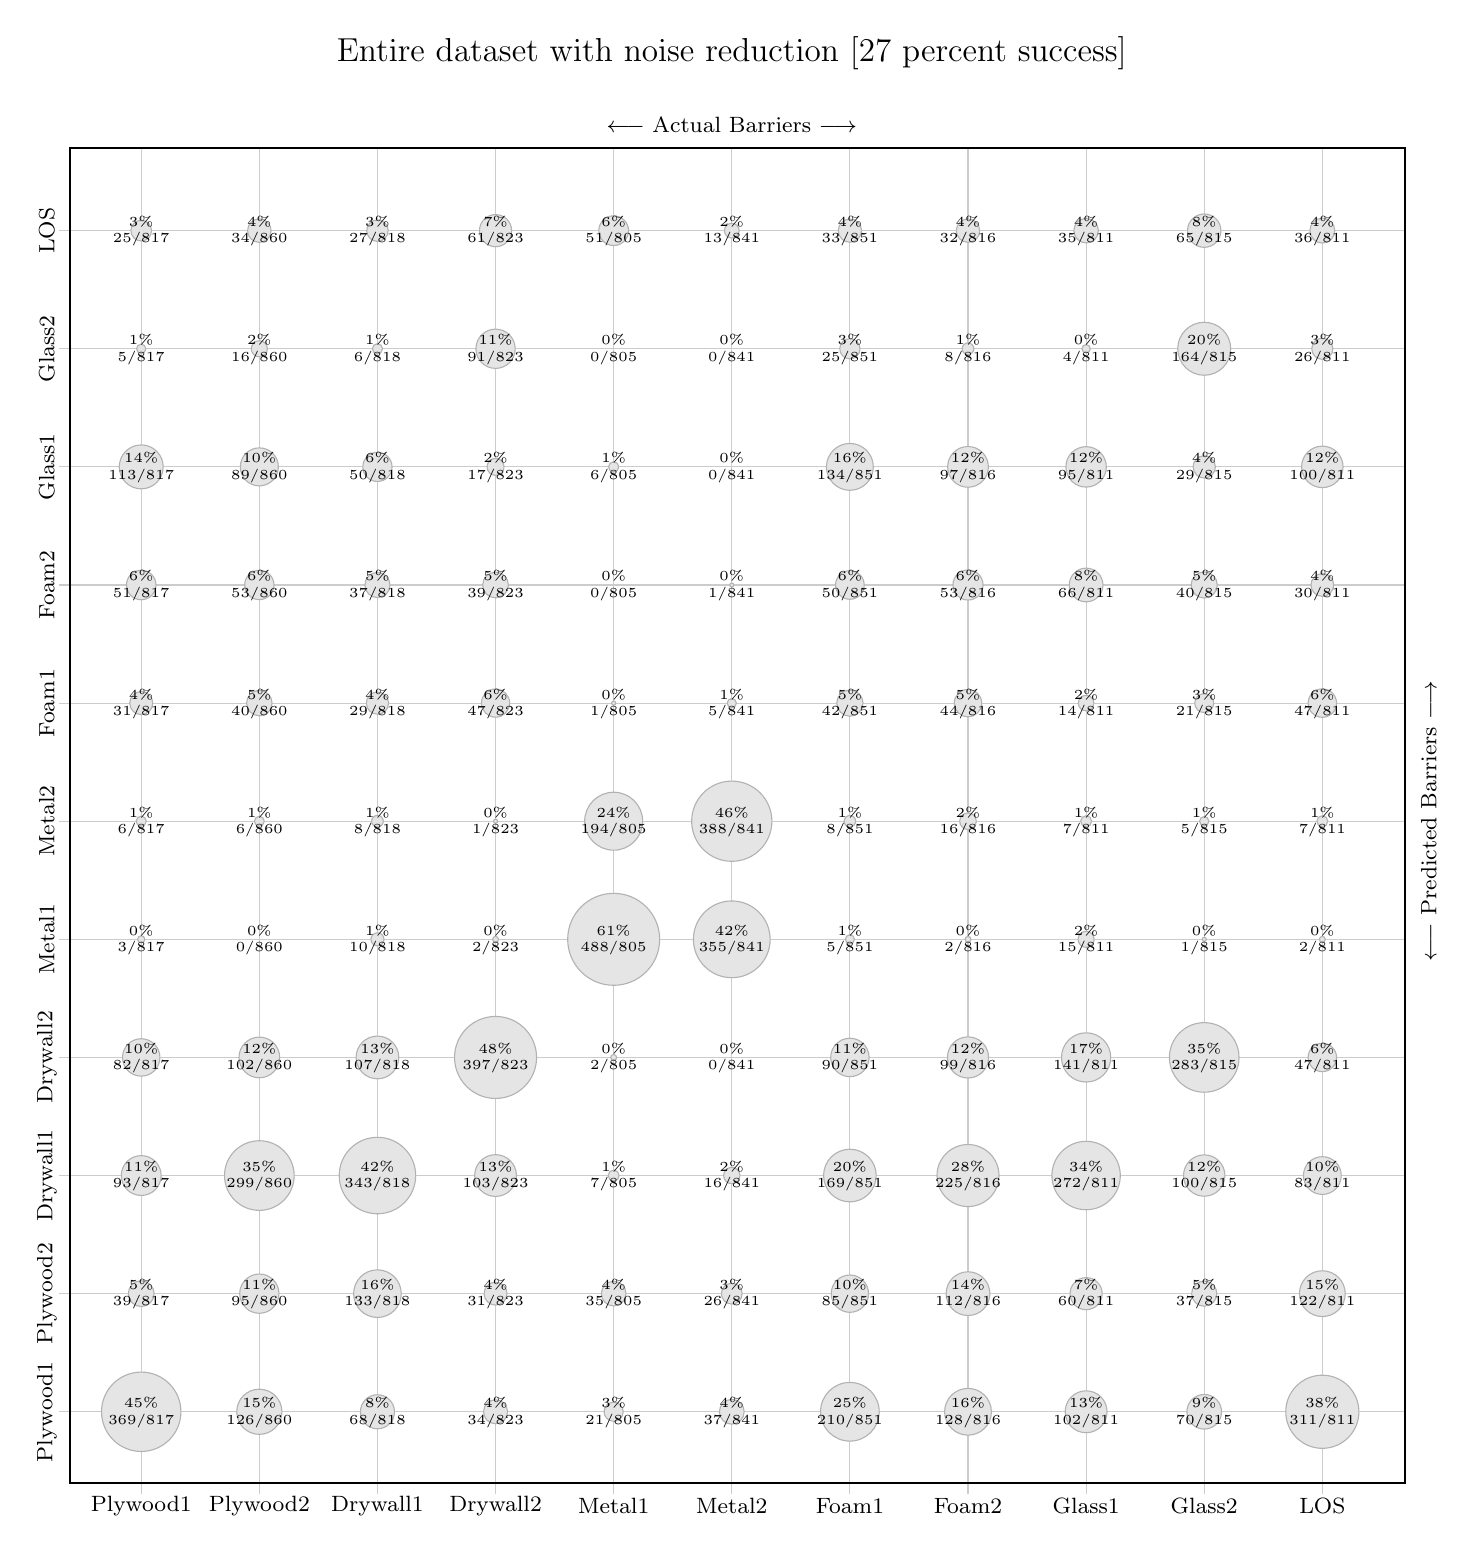
\begin{tikzpicture}
   [scale=1.5, anno/.style={draw=none,fill=none,font=\tiny},
   head/.style={draw=none,fill=none,font=\footnotesize},
   title/.style={draw=none,fill=none,font=\large},
   bubble/.style={draw=black!30, inner sep=0pt, fill=black!10, circle}]{
\draw[step=1cm, black!20, thin] (-.7,-.7) grid (\nbclasses-.3,\nbclasses-.3);
\draw[black,thick] (-.6,-.6) rectangle (\nbclasses-.3,\nbclasses-.3);

\node[title] at (\nbclasses/2-0.5, \nbclasses+.5) {\titletext};
\node[head] at (\nbclasses/2-0.5, \nbclasses-.1) {$\longleftarrow$\ Actual Barriers\ $\longrightarrow$};
\node[head, rotate=90] at (\nbclasses-.1, \nbclasses/2-0.5) {$\longleftarrow$\ Predicted Barriers\ $\longrightarrow$};

\foreach \bar / \iter in \nbviewgraphlabels {
   \node[head] at (\iter,-.8) {\bar};
   \node[head,rotate=90] at (-.8, \iter) {\bar}; }

\foreach \pct / \rad / \x / \y / \num / \tot in \nbviewgraphdata {
   \node[bubble, minimum size=1.5*\rad cm] at (\x,\y) {};
   \node[anno] at (\x,\y+.075) {\pct\%};
   \node[anno] at (\x,\y-.075) {\num/\tot};}
};
\end{tikzpicture}
